Give a short Outline

\section{Setup}
Introduction to this section!

\subsection{Choice of Datasets}
Luis' Taxonomy, verschiedene Bereiche -> TUDataset

\subsection{Choice of Models}
GIN weil sehr expressive \cite{Xu2018}, GAT und GCN wegen \cite{Nikolentzos2023} mit basic pool um complexity der models zu containen und bessere vergleiche zu haben

$\wlnn$ auch nur mit basic pool

\subsection{Experimental Setup}
python 3.10, pytorch und pytorch-geometric (use footnotes from outline). Use of Wheights and Biases as data logging instance, HPC, Colab und meine eigene Hardware - > summierte overall computation time. Standard procedure, training with 10-fold and repition and a split of training, validation and test dataset.

\section{Results}
Introduction to this section!

\subsection{Explain how results look like}
Shortly explain, their performance and how they typically learn. Grafiken über das mean train\_acc, val\_acc, test\_acc vs. epochs.

\subsubsection{1-WL+NN}
Explain most important parameters such as k-wl mit der wl accuracy on. Show how it relates to the datasets by showing the table of theoretical accuracies, 
Grafiken über das mean train\_acc, val\_acc, test\_acc vs. epochs.

\subsubsection{GNN}
Show performance of different GNN models -> Boxplot of different pooling functions
Grafiken über das mean train\_acc, val\_acc, test\_acc vs. epochs.

\subsection{Test Accuracy}
Show a big table with all test-accuracies and its standard deviaton and highlight in bold face, the best one.
Asses the std of both model types.

\begin{table}
    \resizebox{.975\textwidth}{!}{ 	\renewcommand{\arraystretch}{1.05}
		\begin{tabular}{@{}c <{\enspace}@{}lcccccc@{}}	\toprule
			& \multirow{3}{*}{\vspace*{4pt}\textbf{Method}}&\multicolumn{6}{c}{\textbf{Dataset}}\\\cmidrule{3-8}
			& & {\textsc{Enzymes}}         &  {\textsc{Imdb-Binary}}      & {\textsc{Mutag}}           & {\textsc{NCI1}}       & {\textsc{Proteins}}           & 
			{\textsc{Reddit-Binary}}
			\\
			\toprule
			\multirow{6}{*}{\rotatebox{90}{$\wlnn$}} 	&
			\textsf{Max}       &  37.0 \scriptsize	$\pm 1.0$ &   68.1  \scriptsize $\pm 1.7$ & 47.5 \scriptsize $\pm 0.7$ &  85.7 \scriptsize $\pm 1.6$ &  66.9 \scriptsize $\pm 0.3$ &    75.2 \scriptsize $\pm 0.4$
			\\ 
			& \textsf{Mean}               & 42.3   \scriptsize	$\pm 1.1$        & 67.1    \scriptsize $\pm 1.5$           & 46.8  \scriptsize $\pm 0.8$           & 85.4  \scriptsize $\pm 1.5$          & \textsc{Oot}                        & \textsc{Oot}       
			\\ 	
			& \textsf{Sum}     & 55.9  \scriptsize	$\pm 1.0$         & 73.0     \scriptsize $\pm 0.7$          & 50.1 \scriptsize $\pm 0.9$            & 85.6  \scriptsize $\pm 1.4$          & 84.6  \scriptsize $\pm 0.3$         & 75.1 \scriptsize $\pm 0.5$           
			\\  
			\cmidrule{2-8}  		
			& \textsf{Embedding-Max} & 40.5  \scriptsize	$\pm 7.4$         & 69.4  \scriptsize $\pm 4.9$             & 0.0 \scriptsize $\pm 0.0$            & 82.7  \scriptsize $\pm 2.0$          & \textbf{75.2} \scriptsize $\pm 3.9$ & 0.0 \scriptsize $\pm 0.0$        
			\\ 
			& \textsf{Embedding-Mean}     & 42.6 \scriptsize	$\pm 9.0$ & \textbf{72.4}     \scriptsize $\pm 4.1 $         & 0.0 \scriptsize $\pm 0.0$            & 83.1   \scriptsize $\pm 1.9$         & 72.3  \scriptsize $\pm 4.2$         &  0.0 \scriptsize $\pm 0.0$                     
			\\ 
			& \textsf{Embedding-Sum} & \textbf{48.3} \scriptsize	$\pm 8.1$          & 72.0  \scriptsize $\pm 3.8$             & 0.0 \scriptsize $\pm 0.0$            & \textbf{83.6}   \scriptsize $\pm 2.2$         & 75.2  \scriptsize $\pm 4.5$   	& 0.0  \scriptsize $\pm 0.0$                     
			\\ 
			\cmidrule{2-8}
			\multirow{9}{*}{\rotatebox{90}{Graph Neural Networks}} 
			& \textsf{GAT:Max}                    & 31.2 \scriptsize $\pm 6.0$        & 70.7 \scriptsize $\pm 4.8$          & 0.0 \scriptsize $\pm 0.0$            & 58.0 \scriptsize $\pm 4.2$          & 72.5 \scriptsize $\pm 5.1$         & 0.0 \scriptsize $\pm 0.0$  
			\\ 
			& \textsf{GAT:Mean}    & 28.9 \scriptsize $\pm 5.9$          & 70.9 \scriptsize $\pm 3.7$           & 0.0 \scriptsize $\pm 0.0$            & 66.1 \scriptsize $\pm 2.8$         & 64.9 \scriptsize $\pm 6.4$       & 0.0 \scriptsize $\pm 0.0$
			\\ 
			& \textsf{GAT:Sum}                  & \textbf{34.4} \scriptsize $\pm 7.0$          & 72.2 \scriptsize $\pm 4.5$	            & 0.0 \scriptsize $\pm 0.0$            & 69.8 \scriptsize $\pm 2.6$	          & 73.4 \scriptsize $\pm 3.9$
			& 0.0 \scriptsize $\pm 0.0$          
			\\
			
			\cmidrule{2-8}
					
			& \textsf{GCN:Max} & 33.1 \scriptsize $\pm 7.5$ &	73.5 \scriptsize $\pm 4.1$	& 0.0 \scriptsize $\pm 0.0$ & 61.1 \scriptsize $\pm 3.6$ &	69.8 \scriptsize $\pm 5.9$ & 0.0 \scriptsize $\pm 0.0$  
			\\ 
			& \textsf{GCN:Mean} & 29.9 \scriptsize $\pm 5.7$ &	\textbf{74.7} \scriptsize $\pm 3.8$ & 0.0 \scriptsize $\pm 0.0$ &	68.9 \scriptsize $\pm 2.4$ &	70.9 \scriptsize $\pm 5.2$ & 0.0 \scriptsize $\pm 0.0$
			\\ 
			& \textsf{GCN:Sum} & 31.7 \scriptsize $\pm 7.2$ &	73.0 \scriptsize $\pm 4.4$	& 0.0 \scriptsize $\pm 0.0$ & 70.4 \scriptsize $\pm 2.1$ & 3.5 \scriptsize $\pm 3.9$ & 0.0 \scriptsize $\pm 0.0$                        
			\\
			\cmidrule{2-8}	
						
			& \textsf{GIN:Max} & 29.2 \scriptsize $\pm 6.2$	& 70.8 \scriptsize $\pm 4.7$ & 0.0 \scriptsize $\pm 0.0$ & \textbf{79.9} \scriptsize $\pm 2.2$ & \textbf{74.3} \scriptsize $\pm 5.1$ & 0.0 \scriptsize $\pm 0.0$   
			\\ 
			& \textsf{GIN:Mean}  & 31.7 \scriptsize $\pm 6.7$	& 71.1 \scriptsize $\pm 5.4$ & 0.0 \scriptsize $\pm 0.0$ & 	70.8 \scriptsize $\pm 2.2$ & 72.0 \scriptsize $\pm 4.0$ & 0.0 \scriptsize $\pm 0.0$
			\\ 
			& \textsf{GIN:Sum} & 28.9 \scriptsize $\pm 8.7$ & 	69.5 \scriptsize $\pm 4.8$	& 0.0 \scriptsize $\pm 0.0$ & 70.8 \scriptsize $\pm 2.3$ &	73.2 \scriptsize $\pm 4.3$ & 0.0 \scriptsize $\pm 0.0$
			\\
			\bottomrule
		\end{tabular}}
        \caption{Some caption!}
        \label{tab:my_label}                  
\end{table}

\begin{table}
	\resizebox{0.49\textwidth}{!}{ 	\renewcommand{\arraystretch}{1.05}
	\newcommand{\seq}[2]{$(#1, #2)$\text{-}\textsf{SpeqNet}\xspace}
		\begin{tabular}{@{}lcc@{}}	\toprule
			\multirow{3}{*}{\vspace*{4pt}\textbf{Method}}&\multicolumn{2}{c}{\textbf{Dataset}}
			\\
			\cmidrule{2-3} 
			& {\textsc{Alchemy (10k)}} & {\textsc{Zinc?}} 
			\\	
			\toprule
			\textsf{GINE-$\varepsilon^*$}\xspace        & 0.180 {\scriptsize $\pm  0.006$} -1.958  {\scriptsize $\pm  0.047$}
			\\		
			\text{\seq{2}{1}}$^*$   &  0.169 {\scriptsize $\pm 0.005$} -2.010    {\scriptsize $\pm 0.056$}
			\\
			\text{\seq{2}{2}}$^*$    & \textbf{0.115} {\scriptsize $\pm 0.001$} -2.722  {\scriptsize $\pm 0.054$}

			\\
			\cmidrule{1-3}
			\textsf{Embedding-Max} & \textbf{0.305} {\scriptsize $\pm  0.001$} -1.740 {\scriptsize $\pm  0.042$}
			\\
			\textsf{Embedding-Mean} & 0.306 {\scriptsize $\pm  0.001$} -1.720  {\scriptsize $\pm  0.038$}
			\\
			\textsf{Embedding-Sum} & 0.306 {\scriptsize $\pm  0.001$} -1.752  {\scriptsize $\pm  0.022$} 
			\\
			\bottomrule
	\end{tabular}}
	\caption{Mean MAE (mean std.\ MAE, logMAE) on large-scale (multi-target) molecular regression tasks. The results of the models marked $^*$ are taken from \cite{Morris2022}}
\end{table}

\begin{table}
    \resizebox{.975\textwidth}{!}{ 	\renewcommand{\arraystretch}{1.05}
		\begin{tabular}{@{}c <{\enspace}@{}lcccccc@{}}	\toprule
			& \multirow{3}{*}{\vspace*{4pt}\textbf{Method}}&\multicolumn{6}{c}{\textbf{Dataset}}\\\cmidrule{3-8}
			& & {\textsc{Enzymes}}         &  {\textsc{Imdb-Binary}}      & {\textsc{Mutag}}           & {\textsc{NCI1}}       & {\textsc{Proteins}}           & 
			{\textsc{Reddit-Binary}}
			\\
			\toprule
			\multirow{4}{*}{\rotatebox{90}{\small $\wlnn$}}
			& \textsf{Test Accuracy} & 48.3 \scriptsize	$\pm 8.1$ & 72.4 \scriptsize	$\pm 4.1$ &  & 83.6 \scriptsize	$\pm 4.1$ & 75.2 \scriptsize $\pm 3.9$
			\\
			& \textsf{SVM Linear} & 34.37 \scriptsize	$\pm 5.5$ & 71.2 \scriptsize	$\pm 3.9$ &  & 83.4 \scriptsize	$\pm 2.1$ & 73.9 \scriptsize $\pm 4.1$
			\\
			& \textsf{SVM RBF} & 44.97 \scriptsize	$\pm 7.0$ & 72.8 \scriptsize	$\pm 4.3$ &  & 83.6 \scriptsize	$\pm 1.9$ & 75.2 \scriptsize $\pm 4.0$
			\\
			& \textsf{KNN} &  &  &  &  &  & 
			\\
			\cmidrule{2-8}
			\multirow{4}{*}{\rotatebox{90}{\small GNN}}
			& \textsf{Test Accuracy} & 34.4 \scriptsize $\pm 7.0$ &  74.7 \scriptsize $\pm 3.8$ & & 79.9 \scriptsize $\pm 2.2$ & 74.3 \scriptsize $\pm 5.1$
			\\
			& \textsf{SVM Linear} & 33.2 \scriptsize $\pm 5.9$ & 73.9 \scriptsize $\pm 4.2$ & & 67.4 \scriptsize $\pm 2.2$ & 74.7 \scriptsize $\pm 4.2$
			\\
			& \textsf{SVM RBF} & 35.9 \scriptsize $\pm 6.0$ & 74.1 \scriptsize $\pm 3.9$ & & 73.0 \scriptsize $\pm 1.9$ & 74.6 \scriptsize $\pm 4.6$
			\\ 
			& \textsf{KNN} &  &  & &
			\\
			\bottomrule
		\end{tabular}}
        \caption{Some caption!}
        \label{tab:my_label3}                  
\end{table}


\begin{table}
    \resizebox{.975\textwidth}{!}{ 	\renewcommand{\arraystretch}{1.05}
		\begin{tabular}{@{}c <{\enspace}@{}lcccccccc@{}}	\toprule
			& \multirow{3}{*}{\vspace*{4pt}\textbf{1-WL}}&\multicolumn{8}{c}{\textbf{Dataset}}\\\cmidrule{3-10}
			& & {\textsc{Enzymes}}         &  {\textsc{Imdb-Binary}}  & {\textsc{Imdb-Multi}}  & {\textsc{Mutag}}           & {\textsc{NCI1}}       & {\textsc{Proteins}}  & {\textsc{Reddit-Binary}} & {\textsc{Reddit-Multi (5K)}}
			\\
			\toprule
			\multirow{6}{*}{} 	&
			Iterations: $0$       &  81.4 & 60.6 & 44.2 & 93.1 & 91.3 & 91.9 & 83.9 & 55.1
			\\ 
			& Iterations: $1$    & 100.0 & 88.6 & 63.3 & 95.7 & 99.5 & 99.7 & 100.0 & 100
			\\
			& Iterations: $2$    & - & - & - & 99.5 & 99.8 & - & - & -
			\\
			& Iterations: $3$   & - & - & - & 100.0 & 99.8 & - & - & -
			\\
			& Iterations: $4$    & - & - & - & - & - & - & -
			\\
			\cmidrule{2-10}\morecmidrules\cmidrule{2-10}
			& Max Accuracy     & 100.0 & 88.6 & 63.3 & 100.0 & 99.8 & 99.7 & 100.0 & 100.0         
			\\
			\bottomrule
		\end{tabular}}
        \caption{Some caption!}
        \label{tab:my_label2}                  
\end{table}

\begin{figure}
	\centering
	\begin{subfigure}[b]{0.49\textwidth}
		\centering
		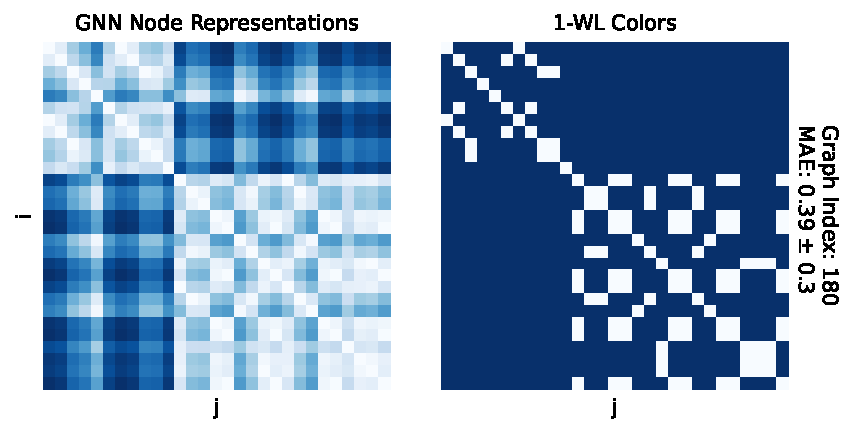
\includegraphics[width=\textwidth]{Figures/heatmaps_ENZYMES_single.pdf}
        \caption{\textsc{Enzymes}}
	\end{subfigure}
	\hfill
	\begin{subfigure}[b]{0.49\textwidth}
		\centering
		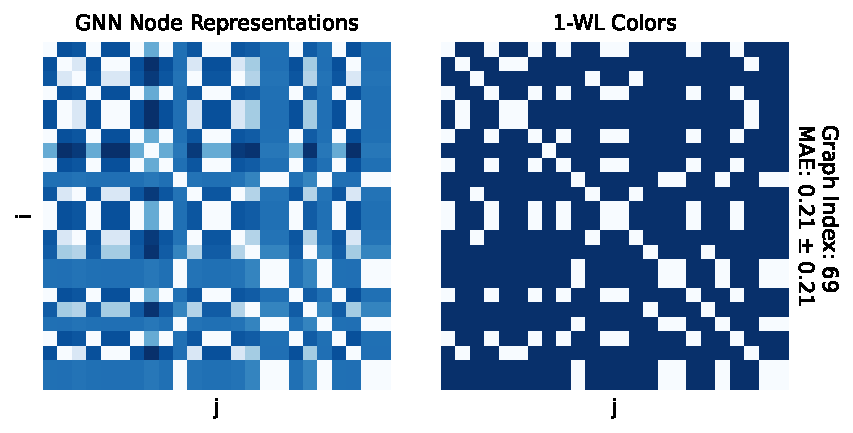
\includegraphics[width=\textwidth]{Figures/heatmaps_IMDB-BINARY_single.pdf}
        \caption{\textsc{Imdb-Binary}}
	\end{subfigure}
	\par\bigskip
	\begin{subfigure}[b]{0.49\textwidth}
		\centering
		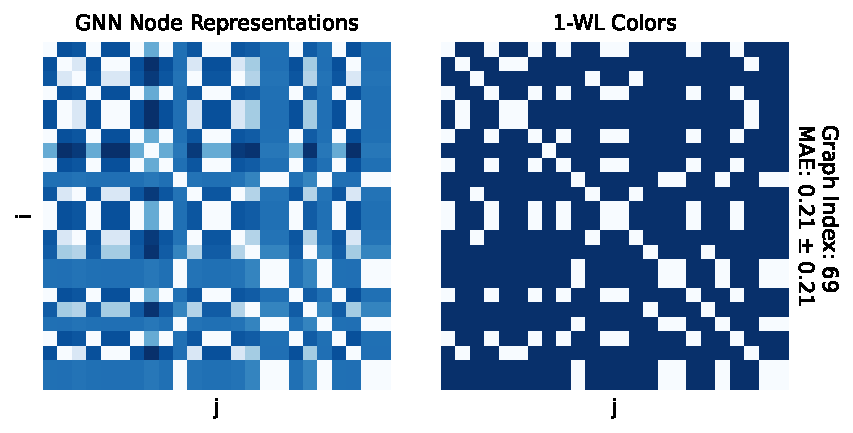
\includegraphics[width=\textwidth]{Figures/heatmaps_IMDB-BINARY_single.pdf}
        \caption{\textsc{Mutag}}
	\end{subfigure}
	\hfill
	\begin{subfigure}[b]{0.49\textwidth}
		\centering
		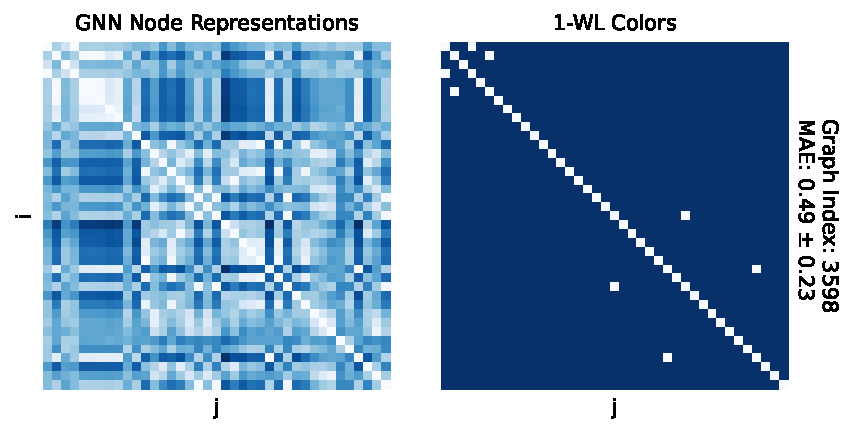
\includegraphics[width=\textwidth]{Figures/heatmaps_NCI1_single.pdf}
        \caption{\textsc{Nci1}}
	\end{subfigure}
	\par\bigskip
	\begin{subfigure}[b]{0.49\textwidth}
		\centering
		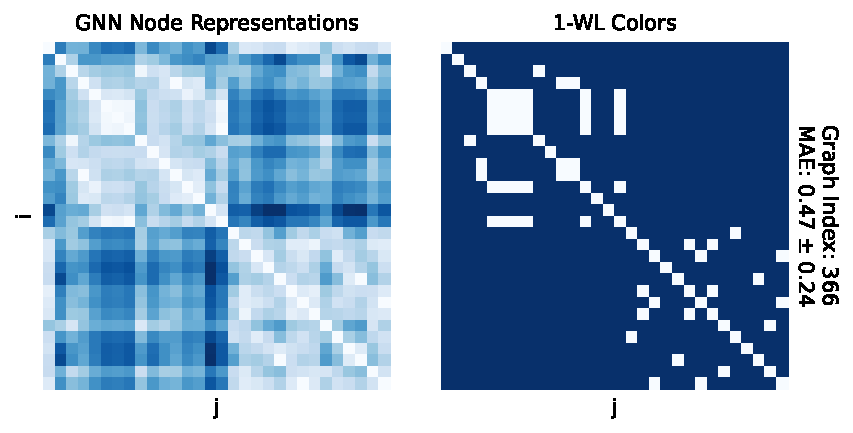
\includegraphics[width=\textwidth]{Figures/heatmaps_PROTEINS_single.pdf}
        \caption{\textsc{Proteins}}
	\end{subfigure}
	\hfill
	\begin{subfigure}[b]{0.49\textwidth}
		\centering
		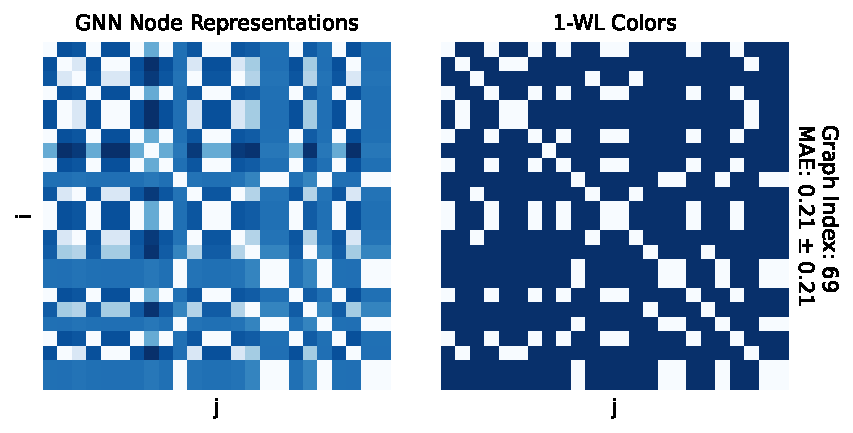
\includegraphics[width=\textwidth]{Figures/heatmaps_IMDB-BINARY_single.pdf}
        \caption{\textsc{Reddit-Binary}}
	\end{subfigure}
	\par\bigskip
	\begin{subfigure}[b]{0.8\textwidth}
		\centering
		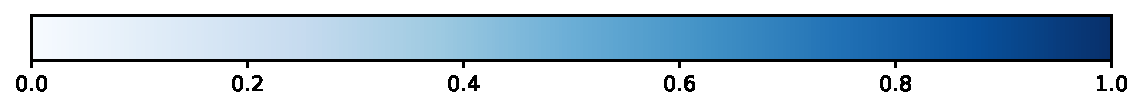
\includegraphics[width=\textwidth]{Figures/colorbar.pdf}
	\end{subfigure}
	\caption{Visualizing the performance of the best performing GNN of each dataset in approximating node colors computed by the 1-WL algorithm.}
\end{figure}

\subsection{Overfitting Behaviour}
Compare the difference between training data performance vs test accuracy accross both models

\subsection{Aggregate Analysis}
Explain what aggregates are and show tSNE with the of the best models with SVM

Also use KNN to assess how good the actuall aggregates are differentiable. -> local clusters ?

\section{Discusssion}
\subsection{Learned Lessons}
\subsection{Future Work}

\section{Conclusion}